\begin{dang}{Tìm điểm cực đại, cực tiểu, giá trị cực đại, giá trị cực tiểu}
 Tìm các điểm cực đại, cực tiểu (nếu có) của hàm số $y=f(x)$.
 \begin{itemize}
 \item \textbf{Bước 1.} Tìm tập xác định $\mathscr{D}$ của hàm số.
 \item \textbf{Bước 2.} Tính đạo hàm $y'=f'(x)$. Tìm các điểm $x_i$, ($i=1,2,3,\ldots,n$) mà tại đó đạo hàm bằng $0$ hoặc không xác định.
 \item\textbf{Bước 3.} Sắp xếp các điểm $x_i$ theo thứ tự tăng dần và lập bảng biến thiên.
 \item \textbf{Bước 4.} Từ bảng biến thiên, suy ra các điểm cực trị (dựa vào nội dung định lý 2).
 \end{itemize}
 \begin{note}
 Cho điểm $A(x_A;y_A)$ và $B(x_B;y_B)$, khi đó
 \begin{itemize}
 \item Độ dài đoạn AB là: $AB=\sqrt{(x_B-x_A)^2 + (y_B-y_A)^2}$.
 \item Phương trình đường $AB$ là: $\dfrac{x-x_A}{x_B-x_A} = \dfrac{y-y_A}{y_B-y_A}$, với $x_A \ne x_B$ và $y_A \ne y_B$.
 \end{itemize}
 \end{note}
\end{dang}
\begin{vd} Tìm các điểm cực trị, cực trị của hàm số
 \begin{listEX}[2]
 \item $y=2x^3-9x^2+12x+3$
 \item $y=\dfrac{x+1}{x-2}$
 \item $y=\dfrac{x^2-3x+3}{x-1}$
 \item $y=\sqrt{4-x^2}$
 \end{listEX}
 \loigiai{}
\end{vd}
\begin{vd}%[2D1Y1-1]
 Tìm các điểm cực trị của hàm số $y=f(x)$, biết
 \begin{listEX}[2]
 \item $f'(x)=x(3x-4)^2(x+2)^3$, $\forall x \in \mathbb{R}$.
 \item $f'(x)=x^2(3x+4)^5(3-x)^4, \forall x\in \mathbb{R}$.
 \item $y=f(x)$ xác định trên $\mathbb{R}\setminus \{2\}$ và~dấu~của~$y'$
 
\begin{tikzpicture}
 \tkzTabInit[lgt=.9,espcl=1.2,deltacl=0.6]
 {$x$ /0.6,$y'$ /0.6}
 {$-\infty$,$-1$,$2$,$3$,$+\infty$}
 \tkzTabLine{,-,$0$,+,d,+,$0$,+,}
 \end{tikzpicture}
 \item	$y=f(x)$ xác định trên $\mathbb{R}$ và dấu của $y'$
 
\begin{tikzpicture}
 \tkzTabInit
 [nocadre=false,lgt=.9,espcl=1.2,deltacl=0.6]
 {$x$/0.6, $y'$/0.6}
 {$-\infty$,$-2 $,$0 $,$2$,$+\infty$}
 \tkzTabLine{, + , d , - , 0 , + , 0, - , }
 \end{tikzpicture}
 \item Đồ thị của $y=f'(x)$ như hình vẽ\\
 \centerline{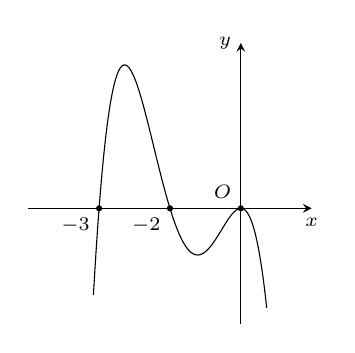
\begin{tikzpicture}[>=stealth,font=\scriptsize,x=1.5cm,y=.7cm]
 \begin{scope}[scale=0.6]
 \draw[->] (-3,0) -- (1,0) node[below] {$x$};
 \draw[->] (0,-3.5) -- (0,5) node[left] {$y$};
 \filldraw (0,0) node[above left=-0.1] {$O$} circle (1.5pt);
 \clip (-3,-3) rectangle (1,5);
 \draw[smooth,samples=100,domain=-2.08:0.4] plot(\x,{-7*(\x)^2*(\x+1)*(\x+2)});
 \filldraw (-2,0) node[below left=-0.1] {$-3$} circle (1.5pt);
 \filldraw (-1,0) node[below left=-0.1] {$-2$} circle (1.5pt);
 \end{scope}
 \end{tikzpicture}}
 \item Đồ thị của $y=f'(x)$ như hình vẽ\\
 \centerline{ 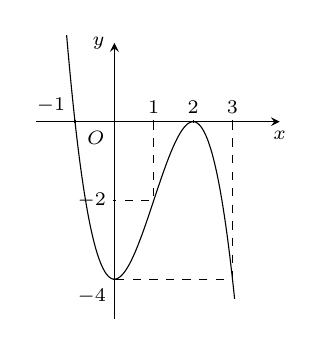
\begin{tikzpicture}[>=stealth,font=\scriptsize]
 \begin{scope}[scale=0.5]
 \def\a{-1} % Hệ số a phải khác 0
 \def\b{3}
 \def\c{0}
 \def\d{-4}
 \draw[->] (-2,0) -- (4.2,0)node[below]{\scriptsize $x$};
 \draw[->] (0,-5) -- (0,2) node[left] {\scriptsize $y$};
 \draw (0,0)node[below left]{\scriptsize $O$};
 \draw (-1,1pt)--(-1,-1pt) node [above left] {$-1$} (1,1pt)--(1,-1pt) node [above] {$1$} (2,1pt)--(2,-1pt) node [above] {$2$} (3,1pt)--(3,-1pt) node [above] {$3$} (-1pt,-2)--(1pt,-2) node [left] {$-2$} (-1pt,-4)--(1pt,-4) node [below left] {$-4$} ;
 \draw[dashed] (1,0)--(1,-2)--(0,-2) (3,0)--(3,-4)--(0,-4);
 \clip (-2,-4.5)rectangle(3.5,2.2);
 \draw[samples=150,smooth,domain=-1.25:5] plot(\x,{\a*(\x)^3+(\b)*(\x)^2+(\c)*\x+(\d)});
 \end{scope}
 \end{tikzpicture}}
 \end{listEX}
 \loigiai{\dotlineEX{25}}
\end{vd}
\begin{vd}%[2D1Y2-2]
 Cho hàm số $y=f(x)$ có đồ thị hoặc bảng biến thiên như hình vẽ
 \begin{itemize}
 \item Xác định các điểm cực trị, các giá trị cực trị của hàm số, các điểm cực trị của đồ thị hàm số.
 \item Tính khoảng cách giữa các điểm cực trị của đồ thị hàm số.
 \item Viết phương trình đường thẳng đi qua hai điểm cực trị của đồ thị hàm số.
 \end{itemize}
 \begin{listEX}[3]
 \item
 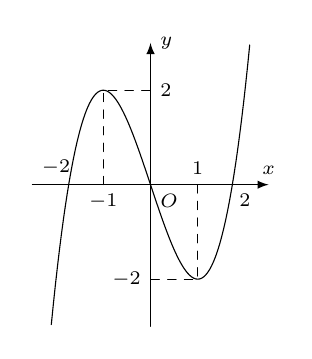
\begin{tikzpicture}[ font=\scriptsize, line join=round, line cap=round, >=stealth]
 \begin{scope}[scale=.6]
 \draw[->,>=latex](-2.5,0)--(2.5,0)node[above]{$x$};
 \draw[->,>=latex](0,-3)--(0,3)node[right]{$y$};
 \node[below right] at (0,0){$O$};
 \clip (-2.6,-3.1) rectangle (2.6,3.1);
 \draw plot [samples=100,domain=-2.1:2.1] (\x,{(\x)^3-3*(\x)});
 \foreach\i in{-1,2}{\node[below] at (\i,0){$\i$};}
 \foreach\i in{2}{\node[right] at (0,\i){$\i$};}
 \foreach\i in{-2}{\node[left] at (0,\i){$\i$};}
 \foreach\i in{1,-2}{\node[above] at (\i,0){$\i$};}
 \draw[dashed](-1,0)--(-1,2)--(0,2)(1,0)--(1,-2)--(0,-2);
 \end{scope}
 \end{tikzpicture}
 \item*
 
\begin{tikzpicture}[font=\scriptsize]
 \begin{scope}[scale=.85]
 \tkzTabInit[nocadre=false,lgt=.9,espcl=2.7,deltacl=0.6]
 {$x$ /0.6,$y'$ /0.6,$y$ /2}
 {$-\infty$,$1$,$2$,$+\infty$}
 \tkzTabLine{,+,$0$,-,d,+,}
 \tkzTabVar{-/$-\infty$, +/$3$,-/$-2$,+/$+\infty$}
 \end{scope}
 \end{tikzpicture}
 \item
 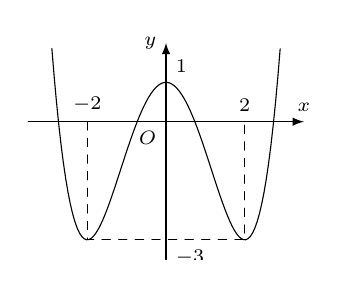
\begin{tikzpicture}[font=\scriptsize, line join=round, line cap=round, >=stealth]
 \begin{scope}[scale=.5]
 \draw[->,>=latex](-3.5,0)--(3.5,0)node[above]{$x$};
 \draw[->,>=latex](0,-3.5)--(0,2)node[left]{$y$};
 \node[below left] at (0,0){$O$};
 \clip (-3.5,-3.5) rectangle (3.5,2);
 \draw plot [samples=100,domain=-2.9:2.9] (\x,{0.25*(\x)^4-2*(\x)^2+1});
 \foreach\i in{-2,2}{\node[above] at (\i,0){$\i$};}
 \foreach\i in{1}{\node[above right] at (0,\i){$\i$};}
 \foreach\i in{-3}{\node[below right] at (0,\i){$\i$};}
 \draw[dashed](-2,0)--(-2,-3)--(2,-3)--(2,0);
 \end{scope}
 \end{tikzpicture}
 \item*
 
\begin{tikzpicture}[font=\scriptsize]
 \begin{scope}[scale=.85]
 \tkzTabInit[nocadre=false,lgt=.9,espcl=2,deltacl=0.6]
 {$x$ /0.6,$y'$ /0.6,$y$ /2}
 {$-\infty$,$-1$,$0$,$1$,$+\infty$}
 \tkzTabLine{,+,d,-,$0$,+,d,-,}
 \tkzTabVar{-/$-\infty$, +/$1$,-/$-1$,+D+/$+\infty$/$+\infty$,-/$-\infty$}
 \end{scope}
 \end{tikzpicture}
 \end{listEX}
 \loigiai{\dotlineEX{63}}
\end{vd}
\BTTN
\Opensolutionfile{ans}[ans/2D1-2-DANG-1]
\begin{ex}%[2D1Y2-2]
 \immini[thm]{Cho hàm số $y=f(x)$ có bảng biến thiên như hình vẽ. Mệnh đề nào dưới đây \textbf{sai}?
 \choice[1]
 {Hàm số có ba điểm cực trị}
 {Hàm số có giá trị cực đại bằng $ 3 $}
 {\True Hàm số có giá trị cực đại bằng $0$}
 {Hàm số có hai điểm cực tiểu}}{	
\begin{tikzpicture}
 \tkzTabInit[espcl=1.5,lgt=1]
 {$x$/0.7,$y'$/0.7,$y$/1.9}
 {$-\infty$,$-1$,$ 0 $,$1$,$+\infty$}
 \tkzTabLine{,-,0,+,0,-,0,+}
 \tkzTabVar{+/$+\infty$,-/$0$,+/$3$,-/$0$,+/$+\infty$}
 \end{tikzpicture}}
 \loigiai{
 Từ bảng biến thiên ta có hàm số có giá trị cực đại bằng $ 3 $.
 }
\end{ex}
%%câu 8
\begin{ex}%[2D1Y2-2]
 \immini[thm]{Cho hàm số $y= f(x)$ có bảng biến thiên như sau. 	Điểm cực đại của hàm số đã cho là
 \choice[2]
 {$x=-4$}
 {$x=7$}
 {$x=-2$}
 {\True $x=6$}}{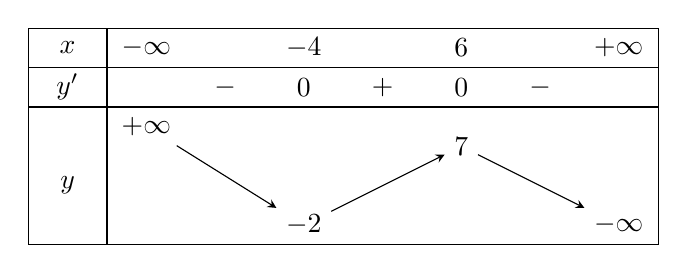
\begin{tikzpicture}[yscale=.5,xscale=1,
 kxd/.pic={\draw[double] (90:.5)--(-90:.5);}]
 \begin{scope}[shift={(-.5,.5)}]
 \draw
 (0,0) rectangle +(8,-5.5)
 (0,-1)--+(0:8) (0,-2)--+(0:8) (1,0)--+(-90:5.5);
 \end{scope}
 \path
 (0,0) node{$x$} % <<< dòng 1
 ++(0:1) node{$-\infty$}
 ++(0:2) node{$-4$}
 ++(0:2) node{$6$}
 ++(0:2) node{$+\infty$}
 (0,-1) node{$y'$} % <<< dòng 2
 ++(0:2) node{$-$}
 ++(0:1) node{$0$}
 ++(0:1) node{$+$}
 ++(0:1) node{$0$}
 ++(0:1) node{$-$}
 (0,-3.5) node{$y$} % <<< dòng 3
 ++(0:1)+(90:1.5) node (A) {$+\infty$}
 ++(0:2)+(-90:1) node (B) {$-2$}
 ++(0:2)+(90:1) node (C) {$7$}
 ++(0:2)+(-90:1) node (D) {$-\infty$};
 \begin{scope}[-stealth]
 \draw (A)--(B);
 \draw (B)--(C);
 \draw (C)--(D);
 \end{scope}
 \end{tikzpicture}}
 \loigiai{
 Dựa vào bảng biến thiên, hàm số đạt cực đại tại điểm $x=6$.}
\end{ex}
%--câu 4
\begin{ex}%[2D1Y2-2]
 \immini[thm]{	Cho hàm số $y=f(x)$ xác định, liên tục trên $\mathbb R$ và có bảng biến thiên như sau. 	Hàm số đã cho có bao nhiêu điểm cực trị?
 \choice[2]
 {$3$}
 {$1$}
 {$0$}
 {\True $2$} }{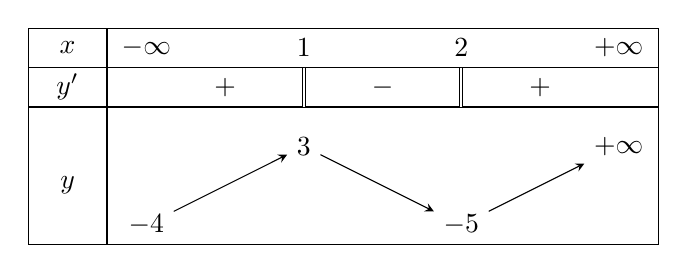
\begin{tikzpicture}[yscale=.5,xscale=1,
 kxd/.pic={\draw[double] (90:.5)--(-90:.5);}]
 \begin{scope}[shift={(-.5,.5)}]
 \draw
 (0,0) rectangle +(8,-5.5)
 (0,-1)--+(0:8) (0,-2)--+(0:8) (1,0)--+(-90:5.5);
 \end{scope}
 \path
 (0,0) node{$x$} % <<< dòng 1
 ++(0:1) node{$-\infty$}
 ++(0:2) node{$1$}
 ++(0:2) node{$2$}
 ++(0:2) node{$+\infty$}
 (0,-1) node{$y'$} % <<< dòng 2
 ++(0:2) node{$+$}
 ++(0:1) pic[scale=.5]{kxd}
 ++(0:1) node{$-$}
 ++(0:1) pic[scale=.5]{kxd}
 ++(0:1) node{$+$}
 (0,-3.5) node{$y$} % <<< dòng 3
 ++(0:1)+(-90:1) node (A) {$-4$}
 ++(0:2)+(90:1) node (B) {$3$}
 ++(0:2)+(-90:1) node (C) {$-5$}
 ++(0:2)+(90:1) node (D) {$+\infty$};
 \begin{scope}[-stealth]
 \draw (A)--(B);
 \draw (B)--(C);
 \draw (C)--(D);
 \end{scope}
 \end{tikzpicture}}
 \loigiai{Từ bảng biến thiên, hàm số đã cho đạt cực đại tại $x=1$ và đạt cực tiểu tại $x=2$, do đó hàm số có hai cực trị.}
\end{ex}
%%câu 5
\begin{ex}%[2D1Y2-2]
 \immini[thm]{Cho hàm số $y=f(x)$ có bảng biến thiên như sau. 	Hàm số đã cho có bao nhiêu cực tiểu?
 \choice[2]
 {$2$}{$1$}{$3$}{\True $0$}}{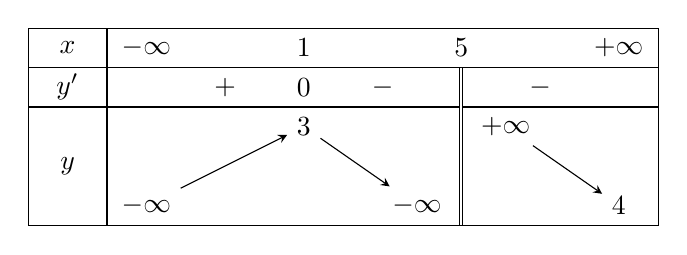
\begin{tikzpicture}[yscale=.5,xscale=1,
 kxd/.pic={\draw[double] (90:.5)--(-90:.5);}]
 \begin{scope}[shift={(-.5,.5)}]
 \draw
 (0,0) rectangle +(8,-5)
 (0,-1)--+(0:8) (0,-2)--+(0:8) (1,0)--+(-90:5);
 \end{scope}
 \path
 (0,0) node{$x$} % <<< dòng 1
 ++(0:1) node{$-\infty$}
 ++(0:2) node{$1$}
 ++(0:2) node{$5$}
 ++(0:2) node{$+\infty$}
 (0,-1) node{$y'$} % <<< dòng 2
 ++(0:2) node{$+$}
 ++(0:1) node{$0$}
 ++(0:1) node{$-$}
 ++(0:1) pic[scale=.5]{kxd}
 ++(0:1) node{$-$}
 (0,-3) node{$y$} % <<< dòng 3
 ++(0:1)+(-90:1) node (A) {$-\infty$}
 ++(0:2)+(90:1) node(B) {$3$}
 ++(0:1)+(-90:1) node[right] (C) {$-\infty$}
 ++(0:1) pic[scale=1.5]{kxd}
 ++(0:1)+(90:1) node[left](D) {$+\infty$}
 ++(0:1)+(-90:1) node(E) {$4$};
 \begin{scope}[-stealth]
 \draw (A)--(B);
 \draw (B)--(C);
 \draw (D)--(E);
 \end{scope}
 \end{tikzpicture}}
 \loigiai{
 Dựa vào bảng biến thiên, hàm số không xác định tại $x=5$ nên $x=5$ không là điểm cực trị. Do đó hàm số có duy nhất một điểm cực đại và hàm số không có điểm cực tiểu.}
\end{ex}
\begin{ex}%[2D1Y2-2]
 \immini[thm]{	Cho hàm số $y=f(x)$ có bảng biến thiên như hình
 vẽ. Tổng các điểm cực đại và điểm cực tiểu của hàm số đã cho bằng
 \choice[2]
 {$5$}
 {\True $ 1 $}
 {$ 4 $ }
 { $ 3 $ }}{
\begin{tikzpicture}
 \tkzTabInit[espcl=2,lgt=1]
 {$x$/0.6,$y'$/0.6,$y$/1.5}
 {$-\infty$,$0$,$1$,$+\infty$}
 \tkzTabLine{,+,0,-,0,+,}
 \tkzTabVar{-/$-\infty$,+/$5$,-/$-1$,+/$+\infty$}
 \end{tikzpicture}}
 \loigiai{
 Dựa vào bảng biến thiên, ta được hàm số đạt cực đại tại $ x=1 $, đạt cực tiểu tại $ x=0 $. Tổng $ 0+1=1 $.
 }
\end{ex}
\begin{ex}%[2D1Y2-2]
 \immini[thm]{	Cho hàm số $y=f(x)$ có bảng biến thiên như hình vẽ. Tổng các điểm cực trị của hàm số đã cho bằng
 \choice[2]
 {$ 2 $}
 {$ 1 $}
 {\True $ -4 $}
 {$ -6 $}}{
\begin{tikzpicture}
 \tkzTabInit[espcl=2,lgt=1]
 {$x$/0.6,$y'$/0.6,$y$/2.0}
 {$-\infty$,$-7$,$ -2 $,$ 3 $,$+\infty$}
 \tkzTabLine{,+,0,-,d,-,0,+,}
 \tkzTabVar{-/$-\infty$,+/$ -4 $,-D+/$-\infty$/$+\infty$,-/$ 6 $,+/$+\infty$}
 \end{tikzpicture}}
 \loigiai{
 Từ bảng biến thiên ta được hàm số đạt cực tiểu tại $ x=3 $, đạt cực đại tại $ x=-7 $. Do đó $ -7+3=-4 $.
 }
\end{ex}
\begin{ex}%[2D1B2-2]
 \immini[thm]{	Cho hàm số $y=f(x)$ có bảng biến thiên như hình vẽ. Khoảng cách giữa điểm cực đại và điểm cực tiểu của đồ thị hàm số đã cho bằng
 \choice[2]
 {$ 3 $}
 {\True $\sqrt{10}$}
 {$\sqrt{2}$}
 { $ 2 $ }}{
\begin{tikzpicture}
 \tkzTabInit[espcl=2,lgt=1]
 {$x$/0.7,$y'$/0.7,$y$/2.2}
 {$-\infty$,$-1$,$0$,$1$,$+\infty$}
 \tkzTabLine{,-,0,+,0,-,0,+}
 \tkzTabVar{+/$+\infty$,-/$0$,+/$3$,-/$0$,+/$+\infty$}
 \end{tikzpicture}}
 \loigiai{
 Dựa vào bảng biến thiên ta được điểm cực đại của đồ thị hàm số là $ (0;3) $. Điểm cực tiểu của đồ thị hàm số là $ (-1;0) $ và $ (1;0) $.\\
 Khoảng cách điểm cực đại và điểm cực tiểu của đồ thị hàm số bằng \[ \sqrt{(0-1)^2+(3-0)^2}=\sqrt{10}. \]
 }
\end{ex}
\begin{ex}%[2D1B2-2]
 \immini[thm]{Cho hàm số $f(x)$ liên tục trên $\mathbb{R}$ và có bảng biến thiên như hình vẽ. Đường thẳng đi qua hai điểm cực trị của đồ thị hàm số đã cho có phương trình
 \choice[2]
 {\True $3y=4x+1$}
 {$3y=x-2$}
 {$3y=13-2x$}
 {$3y=x+2$}}{
\begin{tikzpicture}
 \tkzTabInit[espcl=2,lgt=1]
 {$x$/0.6,$y'$/0.6,$y$/2.2}
 {$-\infty$,$ -1 $,$ 2 $,$5$,$+\infty$}
 \tkzTabLine{,-,0,+,d,-,0,-,}
 \tkzTabVar{+/$+\infty$,-/$ -1 $,+/$ 3 $,R/,-/$-\infty$}
 \tkzTabVal{3}{5}{0.5}{}{$1$}
 \end{tikzpicture}}
 \loigiai{
 Điểm cực tiểu của đồ thị hàm số là $ (-1;-1) $, điểm cực đại của đồ thị hàm số là $ (2;3) $. Đường thẳng qua hai điểm cực trị có dạng $ y=ax+b $. Vì hai điểm cực trị thuộc đường thẳng nên \[ \heva{&-1=a \cdot (-1)+b\\&3=a \cdot 2 +b } \Leftrightarrow \heva{&a=\dfrac{4}{3}\\&b=\dfrac{1}{3}} \Rightarrow y=\dfrac{4}{3}x+\dfrac{1}{3}. \]
 }
\end{ex}
\begin{ex}%[2D1B2-2]
 \immini[thm]{Cho hàm số $y=f(x)$ có đồ thị như hình vẽ bên. Hàm số đã cho đạt cực tiểu tại điểm.
 \choice[2]
 {$x=-1$}
 {$x=1$}
 {\True $x=0$}
 {$x=2$}}{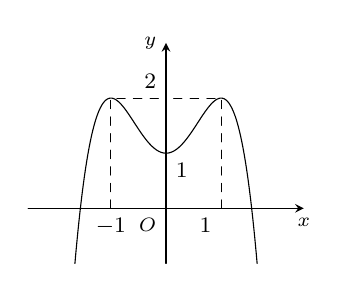
\begin{tikzpicture}[>=stealth,line join=round, line cap=round, font=\footnotesize,scale=0.7]
 \def\a{-1} % Hệ số a phải khác 0
 \def\b{2}
 \def\c{1}
 \draw[->] (-2.5,0) -- (2.5,0) node[below] {\scriptsize $x$};
 \draw[->] (0,-1)--(0,1)node[below right]{$1$} -- (0,3) node[left] {\scriptsize $y$};
 \draw (0,0)node[below left]{\scriptsize $O$};
 \clip (-2.5,-1)rectangle(2.5,2.5);
 \draw[samples=150,smooth,domain=-2:2] plot(\x,{\a*(\x)^4+(\b)*(\x)^2+(\c)});
 \draw[dashed](-1,0)node[below]{$-1$}|-(0,2)node[above left]{$2$};
 \draw[dashed](1,0)node[below left]{$1$}|-(0,2);
 \end{tikzpicture}}
 \loigiai{
 Theo hình vẽ bên hàm số đã cho đạt cực tiểu tại điểm $x=0$.
 }
\end{ex}
\begin{ex}%[2D1B2-2]
 \immini[thm]{Cho hàm số $y=f(x)$ liên tục trên $[a;b]$ và có đồ thị như hình vẽ bên. Số điểm cực đại của hàm số đã cho là
 \choice[2]
 {$4$}
 {$1$}
 {\True $2$}
 {$3$}}{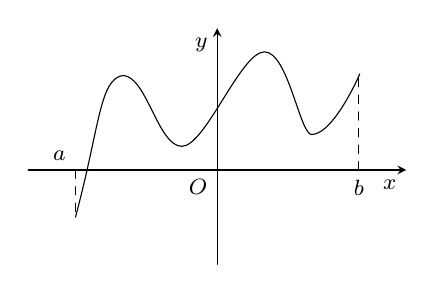
\begin{tikzpicture}[>=stealth,line join=round, line cap=round, font=\footnotesize,scale=0.6]
 \draw[-stealth](-4,0)--(0,0)node[below left]{$O$}--(4,0)node[below left]{$x$};
 \draw[-stealth](0,-2)--(0,3)node[below left]{$y$};
 \draw[dashed]
 (-3,0)node[above left]{$a$}--(-3,-1)
 (3,0)node[below]{$b$}--(3,2)
 ;
 \draw[smooth,black]
 (-3,-1)..controls+(75:2) and+(190:.5)..(-2,2)
 ..controls+(0:.5) and+(180:.5)..(-.75,0.5)
 ..controls+(0:.5)and+(180:.5)..(1,2.5)
 ..controls+(0:.5)and+(180:.25)..(2,.75)
 ..controls+(0:.5)and+(65:.3)..(3,2)
 %..controls+(0:.5)and+(110:.3)..(3,-1.5)
 ;
 \end{tikzpicture}}
 \loigiai{
 Dựa vào đồ thị hàm số đã cho có $2$ điểm cực đại.
 }
\end{ex}
\begin{ex}%[2D1B2-2]
 \immini[thm]{Cho hàm số $y=f(x)$ liên tục trên $[a;b]$ và có đồ thị như hình vẽ bên. Số điểm cực trị của hàm số đã cho là
 \choice[2]
 {\True $4$}
 {$5$}
 {$6$}
 {$3$}}{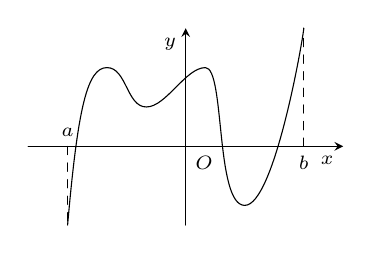
\begin{tikzpicture}[>=stealth,line join=round, line cap=round, font=\scriptsize]
 \begin{scope}[scale=.5]
 \draw[-stealth](-4,0)--(0,0)node[below right]{$O$}--(4,0)node[below left]{$x$};
 \draw[-stealth](0,-2)--(0,3)node[below left]{$y$};
 \draw[dashed]
 (-3,0)node[above]{$a$}--(-3,-2)
 (3,0)node[below]{$b$}--(3,3)
 ;
 \draw[smooth]
 (-3,-2)..controls+(85:3) and+(180:.5)..(-2,2)
 ..controls+(0:.5) and+(180:.5)..(-1,1)
 ..controls+(0:.5)and+(180:.5)..(0.5,2)
 ..controls+(0:.5)and+(180:.75)..(1.5,-1.5)
 ..controls+(0:.75)and+(-95:.3)..(3,3)
 ;
 \end{scope}
 \end{tikzpicture}}
 \loigiai{
 Dựa vào đồ thị ta thấy hàm số đã cho có $4$ điểm cực trị.
 }
\end{ex}
%%==========Câu 50
\begin{ex}%[2D1B2-2]
 \immini[thm]{	Cho hàm số $y=f(x)$ xác định, liên tục trên $[-2;2]$ và có đồ thị như hình vẽ bên. Hàm số $y=f(x)$ đạt cực đại tại
 \choice[2]
 {$x=-2$}
 {\True $x=-1$}
 {$x=1$}
 {$x=2$}}{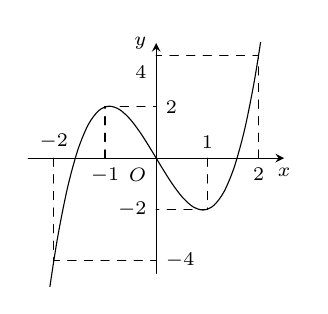
\begin{tikzpicture}[>=stealth,line join=round, line cap=round, font=\scriptsize,yscale=0.5]
 \begin{scope}[scale=0.65]
 \def\a{4/3} % Hệ số a phải khác 0
 \def\b{0}
 \def\c{-10/3}
 \def\d{0}
 \draw[->] (-2.5,0) -- (2.5,0)node[below]{ $x$};
 \draw[->] (0,-4.5) -- (0,4.5) node[left] {$y$};
 \draw (0,0)node[below left]{ $O$};
 \clip (-2.5,-5)rectangle(2.5,4.5);
 \draw[samples=50,smooth,domain=-5:5] plot(\x,{\a*(\x)^3+(\b)*(\x)^2+(\c)*\x+(\d)});
 \draw[dashed](-2,0)node[above]{$-2$}|-(0,-4)node[right]{$-4$};
 \draw[dashed](-1,0)node[below]{$-1$}|-(0,2)node[right]{$2$};
 \draw[dashed](2,0)node[below]{$2$}|-(0,4)node[below left]{$4$};
 \draw[dashed](1,0)node[above]{$1$}|-(0,-2)node[left]{$-2$};
 \end{scope}
 \end{tikzpicture}}
 \loigiai{
 Theo hình vẽ bên hàm số đã cho đạt cực đại tại điểm $x=-1$.
 }
\end{ex}
%%==========Câu 52
\begin{ex}%[2D1B2-2]
 \immini[thm]{	Cho hàm số $y=f(x)$ có đồ thị như hình vẽ bên. Hàm số đã cho đạt cực đại tại điểm.
 \choice[1]
 {\True $x=0$}
 {$x=-1$}
 {$x=2$}
 {$x=3$}}{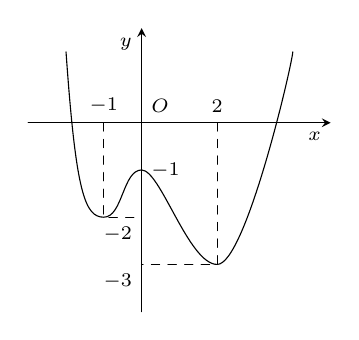
\begin{tikzpicture}[>=stealth,line join=round, line cap=round, font=\scriptsize,x=.8cm]
 \begin{scope}[scale=.6]
 \draw[-stealth](-3,0)--(0,0)node[above right]{$O$}--(5,0)node[below left]{$x$};
 \draw[-stealth](0,-4)--(0,-1)node[ right]{$-1$}--(0,2)node[below left]{$y$};
 \draw[dashed]
 (-1,0)node[above]{$-1$}|-(0,-2)node[below left]{$-2$}
 (2,0)node[above]{$2$}|-(0,-3)node[below left]{$-3$}
 ;
 \draw[smooth,black]
 (-2,1.5)..controls+(-85:3) and+(180:.5)..(-1,-2)
 ..controls+(0:.5)and+(180:.5)..(0,-1)
 ..controls+(0:.5)and+(180:.75)..(2,-3)
 ..controls+(0:.75)and+(-95:.3)..(4,1.5)
 ;
 \end{scope}
 \end{tikzpicture}}
 \loigiai{
 Theo hình vẽ bên hàm số đã cho đạt cực đại tại điểm $x=0$.
 }
\end{ex}
\begin{ex}%[2D1K2-2]
 \immini[thm]{Cho hàm số $y=f(x)$ có đồ thị như hình vẽ bên. Khoảng cách giữa hai điểm cực tiểu của đồ thị hàm số đã cho bằng.
 \choice[1]
 {$3$}
 {\True $\sqrt{10}$}
 {$\sqrt{2}$}
 {$2$}}{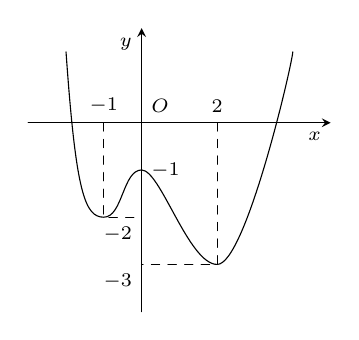
\begin{tikzpicture}[>=stealth,line join=round, line cap=round, font=\scriptsize,x=.8cm]
 \begin{scope}[scale=.6]
 \draw[-stealth](-3,0)--(0,0)node[above right]{$O$}--(5,0)node[below left]{$x$};
 \draw[-stealth](0,-4)--(0,-1)node[ right]{$-1$}--(0,2)node[below left]{$y$};
 \draw[dashed]
 (-1,0)node[above]{$-1$}|-(0,-2)node[below left]{$-2$}
 (2,0)node[above]{$2$}|-(0,-3)node[below left]{$-3$}
 ;
 \draw[smooth,black]
 (-2,1.5)..controls+(-85:3) and+(180:.5)..(-1,-2)
 ..controls+(0:.5)and+(180:.5)..(0,-1)
 ..controls+(0:.5)and+(180:.75)..(2,-3)
 ..controls+(0:.75)and+(-95:.3)..(4,1.5)
 ;
 \end{scope}
 \end{tikzpicture}}
 \loigiai{
 Gọi $A(-1;-2)$ và $B(2;-3)$ là hai điểm cực tiểu của đồ thị hàm số.\\
 $\overrightarrow{AB}=(3;-1)\Rightarrow AB=\sqrt{10}$.
 }
\end{ex}
\begin{ex}%[2D1K2-2]
 \immini[thm]{Cho hàm số $y=f(x)$ có đồ thị như hình vẽ bên. Phương trình đường thẳng đi qua hai điểm cực tiểu của đồ thị hàm số đã cho là.\choice[1]
 {\True $x+3y+7=0$}
 {$x-y+1=0$}
 {$x+y+1=0$}
 {$3x-y-9=0$}}{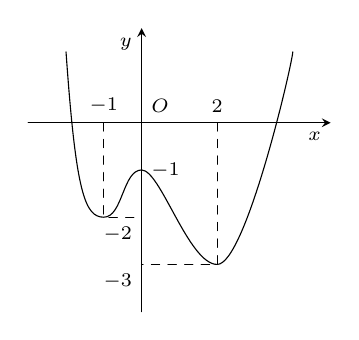
\begin{tikzpicture}[>=stealth,line join=round, line cap=round, font=\scriptsize,x=.8cm]
 \begin{scope}[scale=.6]
 \draw[-stealth](-3,0)--(0,0)node[above right]{$O$}--(5,0)node[below left]{$x$};
 \draw[-stealth](0,-4)--(0,-1)node[ right]{$-1$}--(0,2)node[below left]{$y$};
 \draw[dashed]
 (-1,0)node[above]{$-1$}|-(0,-2)node[below left]{$-2$}
 (2,0)node[above]{$2$}|-(0,-3)node[below left]{$-3$}
 ;
 \draw[smooth,black]
 (-2,1.5)..controls+(-85:3) and+(180:.5)..(-1,-2)
 ..controls+(0:.5)and+(180:.5)..(0,-1)
 ..controls+(0:.5)and+(180:.75)..(2,-3)
 ..controls+(0:.75)and+(-95:.3)..(4,1.5)
 ;
 \end{scope}
 \end{tikzpicture}}
 \loigiai{
 Dựa vào đồ thị ta có $A(-1;-2)$ và $B(2;-3)$ là hai điểm cực tiểu của đồ thị hàm số.\\
 Suy ra phương trình đường thằng đi qua hai điểm $AB$ là $x+3y+7=0$.
 }
\end{ex}
\begin{ex}%[2D1B2-2]
 \immini[thm]{	Cho hàm số $y=f(x)$ xác định trên $\mathbb{R} \setminus \{1\}$ và có bảng xét dấu của đạo hàm như hình vẽ. Hàm số đã cho có bao nhiêu cực trị?
 \choice
 {$0 $}
 {\True $ 1 $}
 {$ 3 $}
 {$ 2 $}	}{
\begin{tikzpicture}
 \tkzTabInit[espcl=1.6,lgt=1]
 {$x$/0.6,$y'$/0.6}
 {$-\infty$,$1$,$2$,$+\infty$}
 \tkzTabLine{,-,d,+,d,-,}
 \end{tikzpicture}}
 \loigiai{Bảng biến thiên:
 \begin{center}
 
\begin{tikzpicture}
 \tkzTabInit[espcl=2.5,lgt=1]
 {$x$/0.6,$y'$/0.6,$y$/1.7}
 {$-\infty$,$1$,$2$,$+\infty$}
 \tkzTabLine{,-,d,+,d,-,}
 \tkzTabVar{+/,-D-/,+/,-/}
 \end{tikzpicture}
 \end{center}
 Từ bảng biến thiên ta có hàm số có một điểm cực đại.
 }
\end{ex}
\begin{ex}%[2D1B2-2]
 \immini[thm]{Cho hàm số $y=f(x)$ xác định trên $\mathbb{R} \setminus \{5\}$ và có bảng xét dấu của đạo hàm như hình vẽ. Hàm số đã cho có bao nhiêu cực trị?
 \choice
 {$4 $}
 {$1 $}
 {$ 3 $}
 {\True $ 2 $ }}{
\begin{tikzpicture}
 \tkzTabInit[espcl=1.2,lgt=1]
 {$x$/0.7,$y'$/0.7}
 {$-\infty$,$1$,$3$,$5$,$+\infty$}
 \tkzTabLine{,-,d,+,0,-,d,+}
 \end{tikzpicture}}
 \loigiai{
 \begin{center}
 
\begin{tikzpicture}
 \tkzTabInit[espcl=2.5,lgt=1.5]
 {$x$/0.7,$y'$/0.7,$y$/1.7}
 {$-\infty$,$1$,$3$,$5$,$+\infty$}
 \tkzTabLine{,-,d,+,z,-,d,+}
 \tkzTabVar{+/$ $,-/,+/$ $,-D-/,+/$ $}
 \end{tikzpicture}
 \end{center}
 Từ bảng biến thiên ta có hàm số có hai điểm cực trị.
 }
\end{ex}
\begin{ex}%[2D1B2-2]
 \immini[thm]{	Cho hàm số $y=f(x)$ có bảng xét dấu của đạo hàm như hình vẽ. Hàm số đã cho đạt cực tiểu tại
 \choice
 {\True $x=0$}
 { $x=2$}
 {$y=0$}
 {$y=2$} }{
\begin{tikzpicture}
 \tkzTabInit[espcl=1.6,lgt=1]
 {$x$/0.6,$y'$/0.6}
 {$-\infty$,$0$,$2$,$+\infty$}
 \tkzTabLine{,-,0,+,0,-,}
 \end{tikzpicture}}
 \loigiai{
 Bảng biến thiên:
 \begin{center}
 
\begin{tikzpicture}
 \tkzTabInit[espcl=2.5,lgt=1.5]
 {$x$/0.6,$y'$/0.6,$y$/1.7}
 {$-\infty$,$0$,$2$,$+\infty$}
 \tkzTabLine{,-,z,+,z,-,}
 \tkzTabVar{+/$ $,-/$ $,+/$ $,-/$ $}
 \end{tikzpicture}
 \end{center}
 Hàm số đạt cực tiểu tại $ x=0 $.
 }
\end{ex}
\begin{ex}%[2D1B2-2]
 Cho hàm số $ f(x) $ có đạo hàm $ f'(x)=x(x-1)^2(x+2)^3 $, $ \forall x \in \mathbb{R} $. Hàm số đã cho đạt cực đại tại
 \choice
 {\True $ x=-2 $}
 {$ x=0 $}
 {$ x=1 $}
 {$ x=2 $}
 \loigiai{
 Ta có $ f'(x)=0 \Leftrightarrow \hoac{&x=0\\&x=1\\&x=-2} $.\\
 Bảng biến thiên.
 \begin{center}
 
\begin{tikzpicture}
 \tkzTabInit[espcl=2.5,lgt=1.5]
 {$x$/0.6,$y'$/0.6,$y$/1.5}
 {$-\infty$,$-2$,$0$,$ 1 $,$+\infty$}
 \tkzTabLine{,+,z,-,z,+,z,+,}
 \tkzTabVar{-/,+/,-/,R/,+/}
 \end{tikzpicture}
 \end{center}
 Từ bảng biến thiên ta được hàm số đạt cực đại tại $ x=-2 $.
 }
\end{ex}
\begin{ex}%[2D1B2-2]
 Cho hàm số $ f(x) $ có đạo hàm $ f'(x)=x^3(x-1)(x-2) $, $ \forall x \in \mathbb{R} $. Điểm cực tiểu của hàm số đã cho là
 \choice
 {\True $ x=0 $ hay $ x=2 $}
 {$ x=2 $}
 {$ x=1 $ hay $ x=2 $}
 {$ x=1 $}
 \loigiai{
 Ta có $ f'(x)=0 \Leftrightarrow \hoac{& x=0\\&x=1\\&x=2.} $\\
 Bảng biến thiên.
 \begin{center}
 
\begin{tikzpicture}
 \tkzTabInit[espcl=2.5,lgt=1.5]
 {$x$/0.7,$y'$/0.7,$y$/2}
 {$-\infty$,$0$,$1$,$2$,$+\infty$}
 \tkzTabLine{,-,z,+,z,-,z,+}
 \tkzTabVar{+/$ $,-/$ $,+/$ $,-/$ $,+/$ $}
 \end{tikzpicture}
 \end{center}
 }
\end{ex}
\begin{ex}%[2D1Y2-1]
 Cho hàm số $y=f(x)$ liên tục trên $\mathbb{R}$, có đạo hàm $f'(x)=x(1-x)^2(3-x)^3(x-2)^4$. Điểm cực tiểu của hàm số $y=f(x)$ là
 \choice
 {$x=2$}
 {$x=3$}
 {$x=1$}
 {\True $x=0$}
 \loigiai
 {
 Bảng xét dấu của $f'(x)=-x(x-1)^2(x-2)^4(x-3)^3$ như hình dưới đây.
 \begin{center}
 
\begin{tikzpicture}
 \tkzTabInit[nocadre=false,lgt=1.2,espcl=2.5,deltacl=0.6]
 {$x$/1, $f'(x)$/1}
 {$-\infty$, $0$, $1$, $2$, $3$, $\infty$}
 \tkzTabLine{,-,0,+,0,+,0,+,0,-,}
 \end{tikzpicture}
 \end{center}
 Từ bảng biến thiên, ta thấy hàm số đạt cực tiểu tại $x=0$, do dấu của $f'(x)$ đổi dấu từ âm sang dương tại $x=0$.
 }
\end{ex}
\begin{ex}%[2D1Y2-1]
 Cho hàm số $y=f(x)$ liên tục trên $\mathbb{R}$ và có đạo hàm $f'(x)=(x+2)(x-1)^{2024}(x-2)^{2023}$. Khẳng định nào đúng?
 \choice
 {Hàm số $y=f(x)$ đạt cực đại tại điểm $x=1$ và đạt cực tiểu tại các điểm $x=\pm2$}
 {Hàm số $y=f(x)$ đồng biến trên mỗi khoảng $(1;2)$ và $(2;+\infty)$}
 {Hàm số $y=f(x)$ có ba điểm cực trị}
 {\True Hàm số $y=f(x)$ nghịch biến trên khoảng $(-2;2)$}
 \loigiai
 {
 Bảng xét dấu của $f'(x)=(x+2)(x-1)^{2020}(x-2)^{2021}$ như hình dưới đây.
 \begin{center}
 
\begin{tikzpicture}
 \tkzTabInit[nocadre=false,lgt=1.2,espcl=2.5,deltacl=0.6]
 {$x$/1, $f'(x)$/1}
 {$-\infty$, $-2$, $1$, $2$, $\infty$}
 \tkzTabLine{,+,0,-,0,-,0,+,}
 \end{tikzpicture}
 \end{center}
 Ta có $f'(x)\le0$, $\forall x\in(-2;2)$ nên hàm số $y=f(x)$ nghịch biến trên khoảng $(-2;2)$.
 }
\end{ex}
\begin{ex}%[2D1Y2-2]
 \immini[thm]{Cho hàm số $f(x)$ có đạo hàm trên $\mathbb{R}$ và đồ thị hàm số $y=f'(x)$ trên $\mathbb{R}$ như hình vẽ. Mệnh đề nào đúng?
 \choice
 {\True Hàm số $y=f(x)$ có $1$ điểm cực đại và $1$ điểm cực tiểu}
 {Hàm số $y=f(x)$ có $2$ điểm cực đại và $2$ điểm cực tiểu}
 {Hàm số $y=f(x)$ có $1$ điểm cực đại và $2$ điểm cực tiểu}
 {Hàm số $y=f(x)$ có $2$ điểm cực đại và $1$ điểm cực tiểu}
 }
 {
 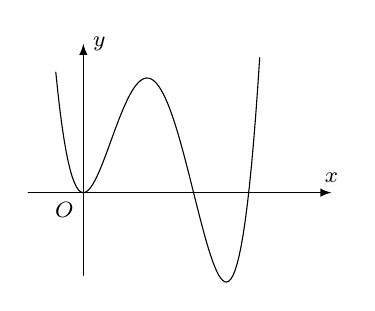
\begin{tikzpicture}[scale=0.7, font=\footnotesize, line join=round, line cap=round, >=stealth]
 \draw[->,>=latex](-1,0)--(4.5,0)node[above]{$x$};
 \draw[->,>=latex](0,-1.5)--(0,2.7)node[right]{$y$};
 \node[below left] at (0,0){$O$};
 \draw plot [samples=100,domain=-0.5:3.2] (\x,{((\x)^2)*(\x-2)*(\x-3)});
 \end{tikzpicture}
 }
 \loigiai
 {
 Ta thấy dấu của $f'(x)$ đổi dấu từ dương sang âm $1$ lần và từ âm sang dương $1$ lần.\\
 Do đó hàm số $f(x)$ có $1$ điểm cực đại và $1$ điểm cực tiểu.
 }
\end{ex}
\begin{ex}%[2D1Y2-2]
 \immini[thm]{Cho hàm số $y=f(x)$ xác định và liên tục trên $\mathbb{R}$ và hàm số $y=f'(x)$ có đồ thị như hình vẽ bên. Khẳng định nào đúng?
 \choice
 {Hàm số $f(x)$ đạt cực đại tại điểm $x=1$}
 {\True Hàm số $f(x)$ đạt cực đại tại điểm $x=0$}
 {Hàm số $f(x)$ đạt cực đại tại điểm $x=-1$}
 {Hàm số $f(x)$ đạt cực đại tại các điểm $x=\pm2$}
 }
 {
 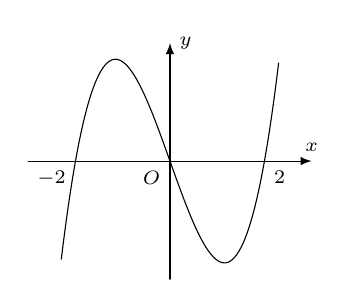
\begin{tikzpicture}[font=\scriptsize, line join=round, line cap=round, >=stealth]
 \begin{scope}[scale=.6]
 \draw[->,>=latex](-3,0)--(3,0)node[above]{$x$};
 \draw[->,>=latex](0,-2.5)--(0,2.5)node[right]{$y$};
 \node[below left] at (0,0){$O$};
 \draw plot [samples=100,domain=-2.3:2.3] (\x,{0.7*((\x)^3-4*(\x))});
 \foreach\i in{-2}{\node[below left] at (\i,0){$\i$};}
 \foreach\i in{2}{\node[below right] at (\i,0){$\i$};}
 \end{scope}
 \end{tikzpicture}
 }
 \loigiai
 {
 Ta thấy $f'(x)$ đổi dấu từ dương sang âm tại điểm $x=0$.\\
 Do đó hàm số $f(x)$ đạt cực đại tại điểm $x=0$.
 }
\end{ex}
\begin{ex}%[2D1Y2-1]
 Hàm số $y=\dfrac{x+1}{2x+1}$ có bao nhiêu điểm cực trị?
 \choice
 {$1$}
 {\True $0$}
 {$2$}
 {$3$}
 \loigiai
 {
 Tập xác định của hàm số là $\mathscr{D}=\mathbb{R}\setminus\left\{\dfrac{-1}{2}\right\}$.\\
 Ta có $y'=\dfrac{2x+1-2(x+1)}{(2x+1)^2}=\dfrac{-1}{(2x+1)^2}<0$, $\forall x\in\mathscr{D}$.\\
 Do đạo hàm không đổi dấu nên hàm số $y=\dfrac{x+1}{2x+1}$ không có điểm cực trị.
 }
\end{ex}
\begin{ex}%[2D1Y2-1]
 Điểm cực tiểu của hàm số $y=x^3-3x^2-9x+2$ là
 \choice
 {$x=11$}
 {\True $x=3$}
 {$x=7$}
 {$x=-1$}
 \loigiai
 {
 Ta có $y'=3x^2-6x-9=3(x-3)(x+1)$. Với $y'=0\Leftrightarrow (x-3)(x+1)=0\Leftrightarrow\hoac{&x=3\\&x=-1.}$\\
 Bảng xét dấu của $y'$ như hình dưới.
 \begin{center}
 
\begin{tikzpicture}
 \tkzTabInit[nocadre=false,lgt=1.2,espcl=2.5,deltacl=0.6]
 {$x$/1, $y'$/1}
 {$-\infty$, $-1$, $3$, $+\infty$}
 \tkzTabLine{,+,0,-,0,+,}
 \end{tikzpicture}
 \end{center}
 Tại $x=3$ đạo hàm đổi dấu từ âm sang dương.\\
 Nên $x=3$ là điểm cực tiểu của hàm số $y=x^3-3x^2-9x+2$.
 }
\end{ex}
\begin{ex}%[2D1Y2-1]
 Cho hàm số $y=-x^4+2x^2-1$. Điểm cực tiểu của hàm số là
 \choice
 {$x=1$}
 {$A(0;1)$}
 {$x=-1$}
 {$x=0$}
 \loigiai
 {
 Ta có $y'=-4x^3+4x$. Với $y'=0\Leftrightarrow -4x(x^2-1)=0\Leftrightarrow\hoac{&x=0\\&x=\pm1.}$\\
 Bảng xét dấu của $y'$ như hình dưới.
 \begin{center}
 
\begin{tikzpicture}
 \tkzTabInit[nocadre=false,lgt=1.2,espcl=2.5,deltacl=0.6]
 {$x$/1, $y'$/1}
 {$-\infty$, $-1$, $0$, $-1$, $+\infty$}
 \tkzTabLine{,+,0,-,0,+,0,-,}
 \end{tikzpicture}
 \end{center}
 Từ bảng xét dấu, ta thấy tại $x=0$ thì $y'$ đổi dấu từ âm sang dương.\\
 Do đó hàm số $y=-x^4+2x^2-1$ có điểm cực tiểu là $x=0$.
 }
\end{ex}
\begin{ex}%[2D1B2-1]
 Cho hàm số $y=\sqrt{x^2-x-20}$. Mệnh đề nào sau đây \textbf{sai}?
 \choice
 {Hàm số nghịch biến trên khoảng $(-\infty;-4)$}
 {Hàm số đạt cực đại tại $x=5$}
 {\True Hàm số đồng biến trên khoảng $(5;+\infty)$}
 {Hàm số không có cực trị}
 \loigiai
 {
 Tập xác định của hàm số $\mathscr{D}=(-\infty;-4]\cup[5;+\infty)$. Ta có $y'=\dfrac{2x-1}{2\sqrt{x^2-x-20}}$.\\
 Với $y'=0\Leftrightarrow \dfrac{2x-1}{2\sqrt{x^2-x-20}}=0\Leftrightarrow x=\dfrac{1}{2}\not\in\mathscr{D}$.\\
 Bảng xét dấu của $y'$ như hình dưới.
 \begin{center}
 
\begin{tikzpicture}
 \tkzTabInit[nocadre=false,lgt=1.2,espcl=2.5,deltacl=0.6]
 {$x$/1, $y'$/1}
 {$-\infty$, $-4$, $5$, $+\infty$}
 \tkzTabLine{,-,,h,,+,}
 \end{tikzpicture}
 \end{center}
 Ta thấy trong khoảng $(5;+\infty)$ thì $y'>0$ nên hàm số đồng biến trên khoảng $(5;+\infty)$.
 }
\end{ex}
%%==========Câu 42
\begin{ex}%[2D1B2-1]
 Khoảng cách giữa hai điểm cực trị của đồ thị hàm số $y=-x^3+3x+2$
 \choice
 {$3\sqrt{5}$}
 {$2\sqrt{3}$}
 {\True $2\sqrt{5}$}
 {$2$}
 \loigiai{
 \begin{enumerate}[$ \star $]
 \item Tập xác định $\mathscr{D}=\mathbb{R}.$
 \item Đạo hàm $y'=-3x^2+3$.
 \item $y'=0\Leftrightarrow \hoac{&x=-1\Rightarrow y=0\\&x=1\Rightarrow y=4}$
 %	\item Giới hạn $\lim\limits_{x\to-\infty}y=+\infty$, $\lim\limits_{x\to+\infty}y=-\infty$.
 \item Bảng biến thiên
 \begin{center}
 
\begin{tikzpicture}[>=stealth,line join=round, line cap=round, font=\footnotesize,scale=0.8]
 \tkzTabInit[nocadre=false,lgt=1.2,espcl=2.5,deltacl=0.6]
 {$x$/0.6,$y'$/0.6,$y$/2}
 {$-\infty$,$-1$,$1$,$+\infty$}
 \tkzTabLine{,-,0,+,0,-,}
 \tkzTabVar{+/$+\infty$,-/$0$,+/$4$,-/$-\infty$}
 \end{tikzpicture}
 \end{center}
 %	\item Hàm số nghịch biến trên $\left(-\infty;-1\right)$ và $\left(1;+\infty\right)$, đồng biến trên $\left(-1;1\right)$.
 \item Hàm số đạt cực đại tại $x=1$, $y_{\textrm{CĐ}}=4$, suy ra $A(1;4)$.
 \item Hàm số đạt cực tiểu tại $x=-1$, $y_{\textrm{CT}}=0$, suy ra $B(-1;0)$.
 \item Khoảng cách giữa hai điểm cực trị của đồ thị hàm số là $AB=\sqrt{(1+1)^2+(4-0)^2}=2\sqrt{5}$.
 \end{enumerate}
 }
\end{ex}
%%==========Câu 43
\begin{ex}%[2D1B2-1]
 Đồ thị hàm số $y=x^3-3x^2-9x+1$ có hai điểm cực trị $A$ và $B$. Điểm nào dưới đây thuộc đường thẳng $AB$?
 \choice
 {$P(1;0)$}
 {$(0;-1)$}
 {\True $N(1;-10)$}
 {$Q(-1;10)$}
 \loigiai{
 \begin{enumerate}[$ \star $]
 \item Tập xác định $\mathscr{D}=\mathbb{R}.$
 \item Đạo hàm $y'=3x^2-6x-9$.
 \item $y'=0\Leftrightarrow \hoac{&x=-1\Rightarrow y=6\\&x=3\Rightarrow y=-26}$
 %	\item Giới hạn $\lim\limits_{x\to-\infty}y=-\infty$, $\lim\limits_{x\to+\infty}y=+\infty$.
 \item Bảng biến thiên
 \begin{center}
 
\begin{tikzpicture}[>=stealth,line join=round, line cap=round, font=\footnotesize,scale=0.8]
 \tkzTabInit[nocadre=false,lgt=1.2,espcl=2.5,deltacl=0.6]
 {$x$/0.6,$y'$/0.6,$y$/2}
 {$-\infty$,$-1$,$3$,$+\infty$}
 \tkzTabLine{,+,0,-,0,+,}
 \tkzTabVar{-/$-\infty$,+/$6$,-/$-26$,+/$+\infty$}
 \end{tikzpicture}
 \end{center}
 \item Hàm số đạt cực đại tại $x=-1$, $y_{\textrm{CĐ}}=6$.
 \item Hàm số đạt cực tiểu tại $x=3$, $y_{\textrm{CT}}=-26$.
 \item Đường thẳng đi qua hai cực trị có dạng $y=ax+b$.\\
 Ta có $\heva{&-a+b=6\\&3a+b=-26}\Leftrightarrow \heva{&a=-8\\&b=-2.}$\\
 Do đó $y=-8x-2$ đi qua điểm $N(1;-10)$.
 \end{enumerate}
 }
\end{ex}
%%==========Câu 44
\begin{ex}%[2D1B2-1]
 Với giá trị thực nào của tham số $m$ để đường thẳng $d\colon y=(2m-1)x+3+m$ vuông góc với đường thẳng đi qua hai điểm cực trị của đồ thị hàm số $y=x^3-3x^2+1$?
 \choice
 {$m=\dfrac{3}{2}$}
 {\True $m=\dfrac{3}{4}$}
 {$m=-\dfrac{1}{2}$}
 {$m=\dfrac{1}{4}$}
 \loigiai{
 \begin{enumerate}[$ \star $]
 \item Tập xác định $\mathscr{D}=\mathbb{R}.$
 \item Đạo hàm $y'=3x^2-6x$.
 \item $y'=0\Leftrightarrow \hoac{&x=0\Rightarrow y=1\\&x=2\Rightarrow y=-3}$
 %	\item Giới hạn $\lim\limits_{x\to-\infty}y=-\infty$, $\lim\limits_{x\to+\infty}y=+\infty$.
 \item Bảng biến thiên
 \begin{center}
 
\begin{tikzpicture}[>=stealth,line join=round, line cap=round, font=\footnotesize,scale=0.8]
 \tkzTabInit[nocadre=false,lgt=1.2,espcl=2.5,deltacl=0.6]
 {$x$/0.6,$y'$/0.6,$y$/2}
 {$-\infty$,$0$,$2$,$+\infty$}
 \tkzTabLine{,+,0,-,0,+,}
 \tkzTabVar{-/$-\infty$,+/$1$,-/$-3$,+/$+\infty$}
 \end{tikzpicture}
 \end{center}
 \item Hàm số đạt cực đại tại $x=0$, $y_{\textrm{CĐ}}=1$.
 \item Hàm số đạt cực tiểu tại $x=2$, $y_{\textrm{CT}}=-3$.
 \item Đường thẳng đi qua hai cực trị có dạng $y=ax+b$.\\
 Ta có $\heva{&b=1\\&2a+b=-3}\Leftrightarrow \heva{&a=-2\\&b=1.}$\\
 Do đó $y=-2x+1$ vuông góc với đường thẳng $d\colon y=(2m-1)x+3+m$ khi và chỉ khi \[(2m-1)\cdot(-2)=-1\Leftrightarrow m=\dfrac{3}{4}.\]
 \end{enumerate}
 }
\end{ex}
\begin{ex}%[2D1K2-1]
 Khoảng cách giữa hai điểm cực trị của đồ thị hàm số $y=\dfrac{x^2-2x+1}{x+1}$ bằng
 \choice
 {\True $4\sqrt{5}$}
 {$4$}
 {$8$}
 {$5\sqrt{2}$}
 \loigiai
 {
 Tập xác định của hàm số là $\mathscr{D}=\mathbb{R}$. Ta có
 \[y'=\dfrac{(2x-2)(x+1)-(x^2-2x+1)}{(x+1)^2}=\dfrac{x^2+2x-3}{(x+1)^2}.\]
 Với $y'=0\Leftrightarrow x^2+2x-3=(x+3)(x-1)=0\Leftrightarrow\hoac{&x=-3\in\mathscr{D}\\&x=1\in\mathscr{D}.}$\\
 Bảng biến thiên của hàm số như hình vẽ.
 \begin{center}
 
\begin{tikzpicture}
 \tkzTabInit[nocadre=false,lgt=1.2,espcl=2.5,deltacl=0.6]
 {$x$/1, $y'$/1, $y$/2}
 {$-\infty$, $-3$, $-1$, $-1$, $\infty$}
 \tkzTabLine{,+,0,-,d,-,0,+,}
 \tkzTabVar{-/$-\infty$, +/$-8$, -D+/$-\infty$/$+\infty$, -/$0$, +/$\infty$}
 \end{tikzpicture}
 \end{center}
 Từ bảng biến thiên, ta thấy hai điểm cực trị của hàm số là $A(-3;-8)$ và $B(-1;0)$.\\
 Khoảng cách giữa hai điểm cực trị là $AB=\sqrt{(-1+3)^2+(0+8)^2}=4\sqrt{5}$.
 }
\end{ex}
\begin{ex}%[2D1B2-1]
 Trong các hàm số sau đây, hàm số nào không có cực trị?
 \choice
 {$y=x^3-3x^2+3$}
 {$y=x^4-x^2+1$}
 {\True $y=x^3+2$}
 {$y=-x^4+3$}
 \loigiai{
 Hàm số $y=x^3+2$ không có cực trị vì $y'=3x^2\ge0$ $\forall x\in \mathbb{R}$.}
\end{ex}
\begin{ex}%[2D1K2-1]
 Hàm số $f(x)=(x-1)(x-2)(x-3)\ldots(x-2020)$ có bao nhiêu điểm cực tiểu?
 \choice
 {\True $1010$}
 {$1009$}
 {$1008$}
 {$2019$}
 \loigiai
 {
 Ta có $\lim\limits_{x\to-\infty}f(x)=+\infty ;\lim\limits_{x\to+\infty}f(x)=+\infty$. Đồ thị hàm số $f(x)$ cắt trục hoành tại $2020$ điểm lần lượt có hoành độ $1,2,3,\ldots,2020$. Đạo hàm $f'(x)$ có $2019$ nghiệm phân biệt lần lượt thuộc các khoảng $(1 ; 2),(2 ; 3),\ldots,(2019 ; 2020)$.\\
 Hàm số có $2019$ điểm cực trị trong đó có $1010$ điểm cực tiểu và $1009$ điểm cực đại.
 }
\end{ex}
\begin{ex}%[2D1K2-2]
 \immini[thm]{Cho hàm số $y=f(x)$ có đạo hàm cấp $2$ trên $\mathbb{R}$ và đồ thị hàm số $y=f''(x)$ là đường cong như hình vẽ bên. Hàm số $y=f(x)$ có tối đa bao nhiêu điểm cực trị?
 \choice[2]
 { $3$}
 { $4$}
 { $1$}
 { \True $2$}
 }{
 \begin{tikzpicture}[font=\footnotesize,line join=round, line cap=round,>=stealth,scale=1]
 \draw[->] (-2.5,0)--(3.5,0) node[above] {$x$};
 \draw[->] (0,-2)--(0,2.5) node[left] {$y$};
 \fill[black] (-2,0)node[below left]{$-2$} circle (1.2pt) (0,0)node[above right]{$O$} circle (1.2pt) (3,0)node[above]{$3$} circle (1.2pt);
 \draw (-2.4,2.5).. controls (-2.3,2) and (-2.2,1) .. (-2,0);
 \draw (-2,0).. controls (-1.5,-2) and (-0.5,-0) .. (0,0);
 \draw (0,0).. controls (1,-0.2) and (1.5,-1) .. (2,-0.9);
 \draw (2,-0.9).. controls (2.5,-0.7) and (2.6,-0.1) .. (3,0);
 \draw (3,0).. controls (3.3,-0.1) and (3.5,-0.5) .. (3.5,-2);
 \end{tikzpicture}
 }
 \loigiai{
 Từ đồ thị hàm số $y=f''(x)$, ta suy ra bảng biến thiên của hàm số $y=f'(x)$
 \begin{center}
 
\begin{tikzpicture}
 \tkzTabInit[nocadre=false,lgt=1.2,espcl=3,deltacl=0.6]
 {$x$/0.7,$f’'(x)$/0.7,$f'(x)$/2}
 {$-\infty$,$-2$,$+\infty$}
 \tkzTabLine{ ,+,$0$,-, }
 \tkzTabVar{-/,+/$f'(-2)$,-/}
 \end{tikzpicture}
 \end{center}
 Từ bảng biến thiên của hàm số $y=f'(x)$, ta thấy đồ thị hàm số $y=f'(x)$ cắt trục hoành tối đa hai tại hai điểm. Suy ra phương trình $f'(x)=0$ có tối đa hai nghiệm và do đó $f'(x)$ đổi dấu tối đa hai lần.\\
 Vậy hàm số $y=f(x)$ có tối đa $2$ điểm cực trị.
 }
\end{ex}
\BTTF
\begin{ex}%[2D1N2-2]
 Cho hàm số $y=f(x)$ có bảng biến thiên. Xét tính đúng, sai của các khẳng định sau
 \begin{center}
 
\begin{tikzpicture}
 \tkzTab
 [lgt=3,espcl=3] % tùy chọn
 {$x$/1, $f’(x)$/1, $f(x)$/2.5} % cột đầu tiên
 {$-\infty$, $-1$, $3$, $+\infty$} % hàng 1 cột 2
 {,+,0,-,0,+,} % hàng 2 cột 2
 {-/ $-\infty$, +/ $7$, -/ $3$ , +/ $+\infty$} % hàng 3 cột 2
 \end{tikzpicture}
 \end{center}
 \choiceTF
 {\True Hàm số $y=f(x)$ có hai cực trị}
 {Hàm số $y=f(x)$ có giá trị cực đại bằng -1}
 {\True Hàm số $y=f(x)$ có điểm cực tiểu là 3}
 {Đồ thị hàm số có điểm cực đại là -1}
 \loigiai{
 \begin{itemchoice}
 \itemch {\bf Đúng}.
 \itemch {\bf Sai}. Hàm số $y=f(x)$ có giá trị cực đại bằng 7.
 \itemch {\bf Đúng}.
 \itemch {\bf Sai}. Đồ thị hàm số có điểm cực đại là $(-1;7)$.
 \end{itemchoice}
 }
\end{ex}
%Câu 2
\begin{ex}%[2D1H2-2]
 Cho hàm số $y=f(x)$ có bảng biến thiên
 \begin{center}
 
\begin{tikzpicture}
 \tkzTab
 [lgt=2,espcl=2.5] % tùy chọn
 {$x$/1, $f’(x)$/1, $f(x)$/2.5} % cột đầu tiên
 {$-\infty$, $-2$, $0$, $2$, $+\infty$} % hàng 1 cột 2
 {,-,0,+,0,-,0,+,} % hàng 2 cột 2
 {+/ $+\infty$, -/ $-4$, +/ $-2$, -/ $-4$ , +/ $+\infty$} % hàng 3 cột 2
 \end{tikzpicture}
 \end{center}
 \choiceTF
 {\True Hàm số $y=f(x)$ có ba cực trị}
 {Hàm số $y=f(x)$ có giá trị cực tiểu bằng -2}
 {\True Hàm số $y=f(x)$ có điểm cực đại là 0}
 {\True Hàm số có hai cực tiểu}
 \loigiai{
 \begin{itemchoice}
 \itemch {\bf Đúng}.
 \itemch {\bf Sai}. Hàm số $y=f(x)$ có giá trị cực tiểu bằng -4.
 \itemch {\bf Đúng}.
 \itemch {\bf Đúng}.
 \end{itemchoice}
 }
\end{ex}
%Câu 3
\begin{ex}%[2D1H2-2]
 Cho hàm số $y=f(x)$ có bảng biến thiên
 \begin{center}
 
\begin{tikzpicture}
 \tkzTab
 [lgt=2,espcl=2] % tùy chọn
 {$x$/0.8, $f’(x)$/0.8, $f(x)$/2} % cột đầu tiên
 {$-\infty$, $1$, $3$, $5$, $+\infty$} % hàng 1 cột 2
 {,-,0,+,d,+,0,-,} % hàng 2 cột 2
 {+/ $+\infty$, -/ $4$, +D-/ $+\infty$ / $-\infty$, +/ $2$, -/ $-\infty$} % hàng 3 cột 2
 \end{tikzpicture}
 \end{center}
 \choiceTF
 {Hàm số $y=f(x)$ có ba cực trị}
 {\True Hàm số $y=f(x)$ có 1 cực đại và 1 cực tiểu}
 {\True Hàm số $y=f(x)$ có điểm cực đại là 5}
 {\True Hàm số $y=f(x)$ có điểm cực tiểu là 1}
 \loigiai{
 \begin{itemchoice}
 \itemch {\bf Sai}. Hàm số $y=f(x)$ có hai cực trị.
 \itemch {\bf Đúng}.
 \itemch {\bf Đúng}.
 \itemch {\bf Đúng}.
 \end{itemchoice}
 }
\end{ex}
%Câu 4
\begin{ex}%[2D1H2-2]
 Cho hàm số $y=f(x)$ có bảng biến thiên
 \begin{center}
 
\begin{tikzpicture}
 \tkzTab
 [lgt=2,espcl=2] % tùy chọn
 {$x$/0.8, $f’(x)$/0.8, $f(x)$/2} % cột đầu tiên
 {$-\infty$, $-2$, $1$, $4$, $+\infty$} % hàng 1 cột 2
 {,-,0,+,d,+,0,-,} % hàng 2 cột 2
 {-/ $-\infty$, +/ $3$, -D-/ $-\infty$ / $-\infty$, +/ $3$, -/ $-\infty$} % hàng 3 cột 2
 \end{tikzpicture}
 \end{center}
 \choiceTF
 {Hàm số $y=f(x)$ có ba cực trị}
 {Hàm số $y=f(x)$ có 2 cực đại và 1 cực tiểu}
 {\True Hàm số $y=f(x)$ có 2 điểm cực đại}
 {Hàm số $y=f(x)$ có 1 điểm cực tiểu}
 \loigiai{
 \begin{itemchoice}
 \itemch {\bf Sai}. Hàm số $y=f(x)$ có hai cực trị.
 \itemch {\bf Sai}. Hàm số có 2 cực đại.
 \itemch {\bf Đúng}.
 \itemch {\bf Sai}. Hàm số không có cực tiểu.
 \end{itemchoice}
 }
\end{ex}
%Câu 5
\begin{ex}%[2D1H2-2]
 Cho hàm số $y=f(x)$ có bảng biến thiên
 \begin{center}
 
\begin{tikzpicture}
 \tkzTab
 [lgt=2,espcl=2] % tùy chọn
 {$x$/0.8, $f’(x)$/0.8, $f(x)$/2} % cột đầu tiên
 {$-\infty$, $1$, $4$, $+\infty$} % hàng 1 cột 2
 {,-,d,+,0,-,} % hàng 2 cột 2
 {-/ $-\infty$, +D-/ $3$ / $-\infty$, +/ $3$, -/ $-\infty$} % hàng 3 cột 2
 \end{tikzpicture}
 \end{center}
 \choiceTF
 {Hàm số $y=f(x)$ không có cực trị}
 {Hàm số $y=f(x)$ có 1 cực đại và 1 cực tiểu}
 { Hàm số $y=f(x)$ có điểm cực đại là 1}
 {\True Hàm số $y=f(x)$ không có điểm cực tiểu}
 \loigiai{
 \begin{itemchoice}
 \itemch {\bf Sai}. Hàm số $y=f(x)$ có một cực trị.
 \itemch {\bf Sai}. Hàm số có 1 cực đại.
 \itemch {\bf Sai}. 1 không phải là điểm cực đại
 \itemch {\bf Đúng}.
 \end{itemchoice}
 }
\end{ex}
\begin{ex}
 Cho hàm số $y=f(x)$ liên tục trên $\mathbb{R}$ và có bảng xét dấu đạo hàm như hình bên.
 \immini{
 \choiceTF
 {Hàm số đồng biến trên khoảng $(-\infty;1)$}
 {\True Hàm số đồng biến trên khoảng $(1;+\infty)$}
 {Hàm số đạt cực đại tại $x=2$}
 {Hàm số có một điểm cực đại và hai điểm cực tiểu}
 }{\vspace{0.1cm}
 
\begin{tikzpicture}
 \tikzset{double style/.append style = {draw=\tkzTabDefaultWritingColor,double=\tkzTabDefaultBackgroundColor,double distance=2pt}}
 \tkzTabInit[nocadre=false, lgt=1, espcl=1.2]{$x$ /0.7,$y'$ /1}{$-\infty$,$0$,$1$,$2$,$+\infty$}
 \tkzTabLine{,+,$0$,-,d,+,$0$,+,}
 \end{tikzpicture}}
 \loigiai{
 Ta có bảng biến thiên như sau:
 \begin{center}
 \begin{tikzpicture}
 \tikzset{double style/.append style = {draw=\tkzTabDefaultWritingColor,double=\tkzTabDefaultBackgroundColor,double distance=2pt}}
 \tkzTabInit[lgt=1.1,espcl=2,nocadre=True]
 {$x$ /.7, $y'$ /.7,$y$ /2}
 {$-\infty$ , $0$, $1$ ,$2$ ,$+\infty$}
 \tkzTabLine{ ,+,$0$,-,d,+,$0$,+, }
 \tkzTabVar{ -/,+/ /,-/,R,+/$+\infty$}
 \end{tikzpicture}
 \end{center}
 Từ đây, suy ra:
 \begin{enumerate}[a)]
 \item Hàm số đồng biến trên khoảng $(-\infty;1)$ là khẳng định sai.
 \item Hàm số đồng biến trên khoảng $(1;+\infty)$ là khẳng định đúng.
 \item Hàm số đạt cực đại tại $x=2$ là khẳng định sai.
 \item Hàm số có một điểm cực đại và hai điểm cực tiểu là khẳng định sai.
 \end{enumerate}
 }
\end{ex}
\begin{ex}
 Cho hàm số $y=x^3-3x^2+4$ có đồ thị $(C)$. Gọi $A$, $B$ là hai điểm cực trị của $(C)$.
 \choiceTF
 {\True Tập xác định của hàm số là $\mathbb{R}$}
 {Hàm số đồng biến trên khoảng $(0;2)$}
 {\True Phương trình đường thẳng qua hai điểm cực trị của đồ thị hàm số là $2x+y-4=0$}
 {\True Diện tích của tam giác $OAB$ bằng $4$, với $O$ là gốc tọa độ}
 \loigiai{
 \begin{enumerate}[a)]
 \item Hàm số đa thức nên có tập xác định là $D=\mathbb{R}$.
 \item Ta có
 \begin{itemize}
 \item [$\bullet$] $y'=3x^2-6x$ và $y'=0 \Leftrightarrow x=0$ hoặc $x=2$.
 \end{itemize}
 Bảng biến thiên:
 \begin{center}
 \begin{tikzpicture}
 \tkzTabInit[lgt=1,espcl=3]
 {$x$ /0.7, $y'$ /0.7, $y$ /2.5}
 {$-\infty$,$0$,$2$,$+\infty$}
 \tkzTabLine{,+,$0$,-,$0$,+,}
 \tkzTabVar{-/$-\infty$,+/$4$,-/$0$,+/$+\infty$}
 \end{tikzpicture}
 \end{center}
 Suy ra hàm nghịch biến trên $(0;2)$.
 \item Tọa độ $A(0;4)$, $B(2;0)$. Phương trình đường thẳng $AB$ là
 $$\dfrac{x-0}{2-0}=\dfrac{y-4}{0-4} \Leftrightarrow 2x+y-4=0$$
 \item Diện tích tam giác vuông $OAB$ là $S_{OAB}=\dfrac{1}{2}OA \cdot OB=4$.
 \end{enumerate}
 }
\end{ex}
\begin{ex}
 Cho hàm số $y=\dfrac{x^2+2x+2}{x+1}$ có đồ thị $(C)$. Gọi $A$, $B$ lần lượt là điểm cực tiểu và điểm cực đại của $(C)$.
 \choiceTF
 {Tập xác định của hàm số là $\mathbb{R}$}
 {Hàm số nghịch biến trên khoảng $(-2;0)$}
 {Tọa độ điểm $A(-2;-2)$, $B(0;2)$}
 {Khoảng cách giữa hai điểm cực trị là $AB=2\sqrt{5}$}
 \loigiai{
 \begin{enumerate}[a)]
 \item Đặt điều kiện mẫu số khác 0, ta được $x+1 \ne 0 \Leftrightarrow x \ne -1$. Suy ra $\mathscr{D}=\mathbb{R}\setminus \left\{-1\right\}$.
 \item $y'=\dfrac{x^2+2x}{(x+1)^2}\Rightarrow y'=0\Leftrightarrow \hoac{& x=-2 \\ & x=0.}$\\
 Ta có bảng xét dấu của hàm $f'(x)$ như sau
 \begin{center}
 \begin{tikzpicture}
 \tkzTabInit[nocadre=false,lgt=1,espcl=3]
 {$x$ /0.7,$y'$ /0.7,$y$ /2}
 {$-\infty$,$-2$,$-1$,$0$,$+\infty$}
 \tkzTabLine{,+,$0$,-,d,-,$0$,+,}
 \tkzTabVar{-/$-\infty$,+/$-2$,-D+/$-\infty$/$+\infty$,-/$2$,+/$+\infty$}
 \end{tikzpicture}
 \end{center}
 Dựa vào bảng xét dấu ta thấy rằng hàm số $y=f'(x)$ nghịch biến trên $(-2;-1)$ và $(-1;0)$.
 \item Tọa độ điểm $A(0;2)$, $B(-2;-2)$
 \item Độ dài $AB=\sqrt{(-2-0)^2+(-2-2)^2}=2\sqrt{5}$.
 \end{enumerate}
 }
\end{ex}
\begin{ex}
 Xét một chất điểm chuyển động dọc theo trục $Ox$. Toạ độ của chất điểm tại thời điểm $t$ được xác định bởi hàm số $x(t)=t^3-6t^2+9t$ với $t\geq 0$. Khi đó $x'(t)$ là vận tốc của chất điểm tại thời điểm $t$, kí hiệu $v(t)$; $v'(t)$ là gia tốc chuyển động của chất điểm tại thời điểm $t$, kí hiệu $a(t)$.
 \choiceTF
 {Phương trình hàm vận tốc là $v(t)=3t^2-6t+9$}
 {\True Phương trình hàm gia tốc là $a(t)=6t-12$}
 {Vận tốc của chất điểm tăng khi $t\in (0;1)$ hoặc $t \in (3;+\infty)$}
 {Vận tốc của chất điểm giảm khi $t\in (1;3)$}
 \loigiai{
 \begin{enumerate}
 \item $v(t)=x'(t)=3t^2-12t+9$
 \item $a(t)=v'(t)=6t-12$.
 \item Xét $v'(t)=6t-12$, $v'(t)=0\Leftrightarrow t=2$\\
 Bảng xét dấu
 \begin{center}
 \begin{tikzpicture}
 \tkzTabInit[nocadre=false,lgt=2,espcl=2.1]
 {$t$ /0.6,$v(t)$ /0.6}
 {$0$,$2$,$+\infty$}
 \tkzTabLine{,-,$0$,+,}
 \end{tikzpicture}
 \end{center}
 Suy ra vận tốc của chất điểm tăng khi $t\in (2;+\infty) $, giảm khi $t\in (0;2)$.
 \end{enumerate}
 }
\end{ex}
\BTTL
\begin{ex}%[2D1N2-2]
 Cho hàm số $y=f(x)$ liên tục trên $\mathbb{R}$ có bảng xét dấu của $f'(x)$ như bên dưới.
 \begin{center}
 \begin{tikzpicture}[scale=1, font=\footnotesize, line join=round, line cap=round, >=stealth]
 \tkzTabInit[nocadre=false, lgt=1.2, espcl=1.8, deltacl=0.6]
 {$x$/0.7, $f'(x)$/0.9}
 {$-\infty$,$-1$,$0$,$2$,$4$,$+\infty$}
 \tkzTabLine{,+,0,-,d,+,0,-,0,+,}
 \end{tikzpicture}
 \end{center}
 Số điểm cực tiểu của hàm số đã cho là bao nhiêu?
 \shortans{$2$}
 \loigiai{Dựa vào bảng xét dấu của $f'(x)$, ta có bảng biến thiên của hàm số là
 \begin{center}
 \begin{tikzpicture}[scale=1, font=\footnotesize, line join=round, line cap=round, >=stealth]
 \tkzTabInit[nocadre=false, lgt=1.2, espcl=1.8, deltacl=0.6]
 {$x$/0.7, $f'(x)$/0.9,$f(x)$/2.2}
 {$-\infty$,$-1$,$0$,$2$,$4$,$+\infty$}
 \tkzTabLine{,+,0,-,d,+,0,-,0,+,}
 \tkzTabVar{-/,+/,-/,+/,-/,+/}
 \end{tikzpicture}
 \end{center}
 Vậy hàm số đã cho có $2$ điểm cực tiểu.}
\end{ex}
\begin{ex}%[2D1H2-2]
 \immini[thm]{
 Cho hàm số $f(x)$ liên tục trên đoạn $[0;3]$ và có đồ thị như hình vẽ bên. Số điểm cực trị của hàm số trên đoạn $[0;3]$ là bao nhiêu?
 }{
 \begin{tikzpicture}[scale=0.5, font=\footnotesize, line join=round, line cap=round, >=stealth]
 \draw[->] (-1,0)--(3.5,0) node[above]{$x$};
 \draw[->] (0,-2.5)--(0,3.5) node[left]{$y$};
 \draw[fill=black] (0,0) circle (1pt) node[below left]{$O$};
 \clip (-1,-2.5) rectangle (3.5,3.5);
 \draw [opacity=0.1] (-1,-2.5) grid (3.5,3.5);
 \draw[smooth,samples=100,domain=0:1] plot(\x,{-(\x)^2});
 \draw[smooth,samples=100,domain=1:2] plot(\x,{-2.5*(\x)^2+6.5*(\x)-5});
 \draw (-0.4,3)--(0,0) (2,-2)--(3,3);
 \foreach \i/\g in {1/-90,2/-90,3/-90} \draw[fill=black] (\i,0) circle(1pt)++(\g:0.3) node{$\i$};
 \foreach \j/\g in {-2/180,-1/180,1/0,2/0,3/0} \draw[fill=black] (0,\j) circle(1pt)++(\g:0.3) node{$\j$};
 \end{tikzpicture}
 }
 \shortans{$3$}
 \loigiai{
 Dựa vào đồ thị ta thấy $f(x)$ đổi chiều biến thiên $3$ lần. \\
 Vậy $f(x)$ có $3$ điểm cực trị.
 }
\end{ex}
\begin{ex}%[2D1N1-2]
    Cho hai hàm số $y=f(x)$, $y=g(x)$ có đồ thị lần lượt được cho ở \textit{Hình} $6a$, \textit{Hình} $6b$. Nêu khoảng đồng biến, nghịch biến và điểm cực trị của mỗi hàm số đó.
    \begin{center}
        \begin{tikzpicture}[scale=.5, font=\footnotesize, line join=round, line cap=round, >=stealth]
            \draw[gray!50,thin,opacity=.5] (-3,-2) grid (4,4);
            \draw[->] (-2.9,0)--(4.1,0) node[below] {$x$};
            \draw[->] (0,-2.1)--(0,4.1) node[left] {$y$};
            \draw (0,0) node [below left] {$O$};
            \foreach \x/\nx in {-1/-1,1/1,2/2}
            \draw[thin] (\x,1pt)--(\x,-1pt) node [below] {$\nx$};
            \foreach \y/\ny in {1/1,2/2}
            \draw[thin] (1pt,\y)--(-1pt,\y) node [left] {$\ny$};
            \begin{scope}
                \clip (-2.8,-2) rectangle (4,4);
                \draw[samples=200,domain=-2.5:-0.32,smooth,variable=\x] plot (\x,{-1.4*(\x)^2-2.92*(\x)-0.51});
                \draw[samples=200,domain=-0.32:0.68,smooth,variable=\x] plot (\x,{2.9*(\x)^2+0.05*(\x)});
                \draw[samples=200,domain=0.68:1.44,smooth,variable=\x] plot (\x,{-5.06*(\x)^2+10.44*(\x)-3.38});
                \draw[samples=200,domain=1.44:3.5,smooth,variable=\x] plot (\x,{4.34*(\x)^2-16.99*(\x)+16.64});
            \end{scope}
            \draw (3.4,2) node{$y=f(x)$};
            \draw (0,-4) node{\text{\textit{Hình }} $6a$};
        \end{tikzpicture}
        \hspace{0.5cm}
        \begin{tikzpicture}[scale=.5, font=\footnotesize, line join=round, line cap=round, >=stealth]
            \draw[gray!50,thin,opacity=.5] (-3,-8.5) grid (3,1);
            \draw[->] (-3,0)--(3,0) node[below] {$x$};
            \draw[->] (0,-8.5)--(0,1) node[left] {$y$};
            \draw (0,0) node [above left] {$O$};
            \foreach \x/\nx in {-2/-2,1/1}
            \draw[thin] (\x,1pt)--(\x,-1pt) node [below] {$\nx$};
            \foreach \y/\ny in {-8/-8}
            \draw[thin] (1pt,\y)--(-1pt,\y) node [left] {$\ny$};
            \begin{scope}
                \clip (-3,-8.6) rectangle (2.9,1.2);
                \draw[samples=200,domain=-2.76:-1.75,smooth,variable=\x] plot (\x,{14.08*(\x)^2+55.22*(\x)+46.11});
                \draw[samples=200,domain=-1.75:0.54,smooth,variable=\x] plot (\x,{-2.4*(\x)^2+0.03*(\x)});
                \draw[samples=200,domain=0.54:1.9,smooth,variable=\x] plot (\x,{2.76*(\x)^2-5.48*(\x)+1.47});
            \end{scope}
            \draw[dashed,thin] (0,-1.25)node[left]{$-\tfrac{5}{4}$}--(1,-1.25);
            \draw (-1,-4) node[rotate=75]{$y=g(x)$};
            \draw (0,-9) node{\text{\textit{Hình }} $6b$};
        \end{tikzpicture}
    \end{center}
    \shortans{}
    \loigiai{
        \begin{itemize}
            \item Quan sát đồ thị \textit{Hình} $6a$, ta thấy hàm số $y=f(x)$ đồng biến trên các khoảng $(-\infty;-1)$, $(0;1)$, $(2;+\infty)$; nghịch biến trên các khoảng $(-1;0)$, $(1;2)$.\\
            Hàm số đạt cực đại tại $x=-1$, $x=1$ và đạt cực tiểu tại $x=0$, $x=2$.
            \item Quan sát đồ thị \textit{Hình} $6b$, ta thấy hàm số $y=g(x)$ đồng biến trên các khoảng $(-2;0)$, $(1;+\infty)$; nghịch biến trên các khoảng $(-\infty;-2)$, $(0;1)$.\\
            Hàm số đạt cực đại tại $x=0$ và đạt cực tiểu tại $x=-2$, $x=1$.
        \end{itemize}
    }
\end{ex}
\begin{ex}%[2D1V2-2]
 \immini[thm]
 {
 Cho hàm số $y=f(x)=x^3+ax^2+bx+c$ có bảng biến thiên như hình vẽ bên. Tính giá trị của biểu thức $P=a+b+3c$.
 }
 {
 \begin{tikzpicture}
 \tkzTabInit[lgt=1.2,espcl=3]
 {$x$ /.7, $y'$ /.7, $y$ /2}
 {$-\infty$,$-1$,$3$,$+\infty$}
 \tkzTabLine{ ,+,z,-,z,+, }
 \tkzTabVar{-/$-\infty$,+/$a-b+c-1$,-/$-24$,+/$+\infty$}
 %	\begin{scope}[on background layer]\path[white]node{MDD372};\end{scope}
 \end{tikzpicture}
 }
 \shortans{$-3$}
 \loigiai{
 Từ bảng biến thiên, ta thấy $x=-1$ và $x=3$ là hai điểm cực trị nên $\heva{&f'(-1)=0\\&f'(3)=0}$ mà $f'(x)=3x^2+2ax+b$.\\
 Do đó $\heva{&2a+b=-3\\&-6a+b=-27}\Leftrightarrow \heva{&a=-3\\&b=-9.}$\\
 Mặt khác $f(3)=-24\Leftrightarrow 9a+3b+c+27=-24\Leftrightarrow c=-51-9a-3b=3.$\\
 Vậy $P=a+b+3c=-3.$
 }
\end{ex}

\begin{ex}%[TeX hóa SGK CTST 12]%[Nguyễn Tiến]%[2D1V1-2]%[2D1V2-2]
 \immini[thm]{
 Đạo hàm $f'(x)$ của hàm số $y=f(x)$ có đồ thị như Hình $12$. Xét tính đơn điệu và tìm điểm cực trị của hàm số $y=f(x)$.
 }{
 \begin{tikzpicture}[scale=0.7, font=\footnotesize, line join=round, line cap=round, >=stealth]
 \def\a{0.125} \def\b{-0.625} \def\c{0.25} \def\d{1} % Hệ số
 \def\xt{-3} \def\xp{6} \def\yt{2.5} \def\yd{-3} % x_trái, x_phải, y_trên, y_dưới (giới hạn)
 \draw[->] (\xt,0)--(\xp,0) node [below]{$x$};
 \draw[->] (0,\yd)--(0,\yt) node [left]{$y$};
 \node at (0,0) [below right]{$O$};
 \clip (\xt+0.1,\yd-1) rectangle (\xp-0.1,\yt-0.1);
 \draw[thick,red,smooth,samples=300,domain=-2:5] plot(\x,{\a*(\x)^3+\b*(\x)^2+\c*(\x)+\d}) node [below left]{$y=f'(x)$};
 \draw[dashed] (-2,0) node [below left]{$-2$} -- (-2,-3);
 \draw[dashed] (5,0) node [below]{$5$} -- (5,2.25);
 \fill (-1,0) circle (1.5pt) node[below right]{$-1$};
 \fill (2,0) circle (1.5pt) node[below left]{$2$};
 \fill (4,0) circle (1.5pt) node[below right]{$4$};
 \node at (1.5,-3.5){\textit{Hình 12}};
 \end{tikzpicture}
 }
\shortans{}
 \loigiai{
 Từ đồ thị ta thấy $f'(x)=0 \Leftrightarrow \hoac{& x=-1\\& x=2\\& x=4.}$\\
 Ta có bảng biến thiên như sau
 \begin{center}
 \begin{tikzpicture}
 \tkzTabInit[nocadre=true,lgt=1.2,espcl=2.5,deltacl=0.6]
 {$x$ /0.6,$f'(x)$ /0.6,$f(x)$ /2}
 {$-2$,$-1$,$2$,$4$,$5$}
 \tkzTabLine{,-,$0$,+,$0$,-,$0$,+,}
 \tkzTabVar{+/,-/,+/,-/,+/}
 \end{tikzpicture}
 \end{center}
 Vậy hàm số đồng biến trên $(-1;2)$ và $(4;5)$, nghịch biến trên $(-2;-1)$ và $(2;4)$.\\
 Hàm số đạt cực đại tại $x=2$ và đạt cực tiểu tại $x=-1$, $x=4$.
 }
\end{ex}
\begin{ex}%[TeX hóa SGK CTST 12]%[Nguyễn Tiến]%[2D1H1-2]%[2D1H2-2]
 Tìm các khoảng đơn điệu và cực trị của các hàm số có đồ thị cho ở Hình $11$.
 \begin{center}
 \begin{tikzpicture}[scale=0.6, font=\footnotesize, line join=round, line cap=round, >=stealth]
 \def\xt{-2} \def\xp{6} \def\yt{4} \def\yd{-1.8} % x_trái, x_phải, y_trên, y_dưới (giới hạn)
 \draw[->] (\xt,0)--(\xp,0) node [below]{$x$};
 \draw[->] (0,\yd)--(0,\yt) node [left]{$y$};
 \node at (0,0) [below right]{$O$};
 \clip (\xt+0.1,\yd-1) rectangle (\xp-0.1,\yt-0.1);
 \draw[smooth,samples=300,thick,red,domain=-1:5] plot(\x,{31/180*(\x)^4-62/45*(\x)^3+97/36*(\x)^2+11/45*(\x)-1});
 \draw[dashed] (-1,0) node [below]{$-1$} -- (-1,3) -- (0,3) node [above left]{$3$} -- (5,3) -- (5,0) node [below]{$5$};
 \draw[dashed] (0,2) node [left]{$2$} -- (2,2) -- (2,0) node [below]{$2$};
 \draw[dashed] (0,-1) node [below left]{$-1$} -- (4,-1) -- (4,0) node [above]{$4$};
 \foreach \x/\y in {-1/3,0/-1,2/2,4/-1,5/3}
 \fill (\x,\y) circle (1.5pt);
 \node at (2,-2.2){\text{a)}};
 \end{tikzpicture}
 \qquad\qquad
 \begin{tikzpicture}[scale=0.5, font=\footnotesize, line join=round, line cap=round, >=stealth]
 \draw[->] (-4,0) -- (4,0) node[below] {$x$};
 \draw[->] (0,-2.5) -- (0,5) node[left] {$y$};
 \node at (0,0) [below right]{$O$};
 \coordinate (A) at (-3,-2);
 \coordinate (B) at (-1,3);
 \coordinate (C) at (0,1);
 \coordinate (D) at (1,-1);
 \coordinate (E) at (3,4);
 \draw[thick,red]
 (A) .. controls +(80:0) and +(180:.8) ..
 (B) .. controls +(0:.3) and +(180:.8) ..
 (C) .. controls +(0:.8) and +(180:.2) ..
 (D) .. controls +(0:0) and +(180:0) .. (E);
 \foreach \x/\y in {-3/-2,-1/3,1/-1,3/4}
 \fill (\x,\y) circle (1.5pt);
 \draw[dashed] (-3,0)node[below left] {$-3$}--(-3,-2)--(0,-2)node[right] {$-2$} (-1,0)node[below] {$-1$}--(-1,3)--(0,3)node[right] {$3$} (1,0)node[above] {$1$}--(1,-1)--(0,-1)node[left] {$-1$} (3,0)node[below] {$3$}--(3,4)--(0,4)node[left] {$4$};
 \node at (0,-3){\text{b)}};
 \end{tikzpicture}
 \\
 \centering \text{\textit{Hình 11}}
 \end{center}
\shortans{}
 \loigiai{
 Từ hình vẽ, ta thấy
 \begin{enumerate}
 \item Hàm số đồng biến trên khoảng $(0;2)$ và $(4;5)$, nghịch biến trên khoảng $(-1;0)$ và $(2;4)$.\\
 Hàm số đạt cực đại tại $x=2$, $y_{\text{CĐ}}=2$; hàm số đạt cực tiểu tại $x=0$ và $x=4$, $y_{\text{CT}}=-1$.
 \item Hàm số đồng biến trên các khoảng $(-3;-1)$ và $(1;3)$, nghịch biến trên khoảng $(-1;1)$.\\
 Hàm số đạt cực đại tại $x=-1$, $y_{\text{CĐ}}=3$; hàm số đạt cực tiểu tại $x=1$, $y_{\text{CT}}=-1$.
 \end{enumerate}
 }
\end{ex}
\begin{ex}%[TeX hóa SGK CTST 12]%[Nguyễn Tiến]%[2D1H2-1]
 Một phần lát cắt của dãy núi có độ cao tính bằng mét được mô tả bởi hàm số
 $$y=h(x)=-\dfrac{1}{1\,320\,000}x^3+\dfrac{9}{3\,520}x^2-\dfrac{81}{44}x+840, \text { với } 0\leq x\leq 2\,000.$$
 Tìm tọa độ các đỉnh của lát cắt dãy núi trên đoạn $[0; 2\,000]$.
 \begin{center}
 \begin{tikzpicture}[font=\footnotesize, line join=round, line cap=round, >=stealth,scale=0.45,transform shape]
 \def\xmin{-20} \def\xmax{14}
 \def\ymin{-1.25} \def\ymax{7.75}
 \clip (\xmin-.1,\ymin-.1) rectangle (\xmax+.1,\ymax+.1);
 \fill[orange!20] (-18,0)..controls +(0:2) and +(178:4) ..(-9.5,1)
 ..controls +(2:2) and +(178:4) ..(-4.3,1.5)
 ..controls +(45:2) and +(130:2) ..(0,2.3)
 ..controls +(-50:.5) and +(160:.5) ..(1.3,1.2)
 ..controls +(-20:1.5) and +(150:2) ..(6,4)
 ..controls +(-30:1.5) and +(135:2) ..(8.5,1.8)
 ..controls +(-40:1.5) and +(155:2) ..(12 ,0)--cycle
 ;
 \draw[thick,red] (0,2.3)
 ..controls +(-50:.5) and +(160:.5) ..(1.3,1.2)
 ..controls +(-20:1.5) and +(150:2) ..(6,4);
 \draw[->] (\xmin,0)--(\xmax,0) node [below left]{\Huge $x$};
 \draw[->] (0,\ymin)--(0,\ymax) node [below left]{\Huge $y$};
 \node at (0,0) [below left]{\Huge $O$};
 \node at (4.2,4.3) [thick,red,above]{\Huge $y=h(x)$};
 \draw[dashed](6,4)--(6,0) node[below] {\Huge $2\,000$};
 \foreach \y/\diem in {1.5/500,3/1\,000,4.5/1\,500,6/2\,000}
 \draw[shift={(0,\y)},color=black] (5pt,0pt) -- (-5pt,0pt) node[left]{\Huge $\diem$};
 \end{tikzpicture}
 \end{center}
\shortans{$\left(450; \dfrac{7365}{16}\right)$, và $\left(1\,800, \dfrac{15\,315}{11}\right)$}
 \loigiai{
 Trên đoạn $[0; 2\,000]$, ta có $y'=-\dfrac{1}{440\,000}x^2+\dfrac{9}{1\,760}x^2-\dfrac{81}{44}$.\\
 Suy ra $y'=0 \Leftrightarrow \hoac{& x=450\\& x=1800.}$\\
 Bảng biến thiên
 \begin{center}
 \begin{tikzpicture}
 \tkzTabInit[nocadre=true,lgt=1.2,espcl=3,deltacl=0.6]
 {$x$ /0.6,$y'$ /0.6,$y$ /2}
 {$0$,$450$,$1800$,$2000$}
 \tkzTabLine{,-,$0$,+,$0$,-,}
 \tkzTabVar{+/$840$,-/$\dfrac{7365}{16}$,+/$\dfrac{15\,315}{11}$,-/$\dfrac{43720}{33}$}
 \end{tikzpicture}
 \end{center}
 Vậy tọa độ các đỉnh là $\left(450; \dfrac{7365}{16}\right)$, và $\left(1\,800, \dfrac{15\,315}{11}\right)$.
 }
\end{ex}
\Closesolutionfile{ans}
%\indapan{10}{ans/2D1-2-DANG-1}